\section{Aspectos Gerais do Funcionamento do Sistema}

Tendo em vista que o sistema a ser projetado é um sistema crítico, deve-se escolher os dispositivos de forma que haja redundância, ou seja, em caso de falha de algum dispositivo, existe outro que poderá coletar as mesmas informações. Para fazer a comunicação interveicular, foi escolhido o Transponder, para identificar a intenção de ultrapassagem, será usado como parâmetro as informações do sensor de movimento angular, da câmera e a ativação da seta, sendo este último um fator que pode ocorrer ou não. Para verificar a viabilidade de ultrapassagem, será utilizado o GPS, o Radar e o Lidar.

\section{Funcionamento do sistema}

Condições iniciais do sistema:

\begin{itemize}
	\item Microprocessador em modo de baixo consumo;
	\item Sensor de posição angular ativado;
	\item Câmera ativada;
	\item Lidar e radar ativados;
	\item GPS ativado;
	\item Transponder ativado.
\end{itemize}

A identificação da intenção de ultrapassagem se dará da seguinte maneira:

\begin{enumerate}

\item Microprocessador monitora os dados, todos os itens a seguir serão analisados pelo processador:

\begin{enumerate}
	\item Verificar seta (pode ser ativada ou não);
	\item Ler informação do sensor de posição angular, detectar o giro do volante, se a posição angular mudar, condição de possível ultrapassagem identificada;
	\item Câmera, faz a identificação da mudança de faixa, se sim condição de possível ultrapassagem identificada;
	\item Câmera, Lidar e Radar identificam a diminuição da distância com o carro da frente, se sim condição de possível ultrapassagem identificada, se estiver muito próximo, acionar alarme, se não buscar informação do transponder.
\end{enumerate}

\item Caso seja identificada a intenção de ultrapassagem, o microprocessador coletará informações da câmera, do radar e do lidar, para identificar a distância do carro em sentido contrário, caso seja menor que 200 m, a ultrapassagem será de curta distância, caso contrário será de longa distância. Tendo isso em vista, o processador coletará mais informações dos dispositivos para validar a ultrapassagem.

Validação da ultrapassagem preventiva, ou seja, para longas distâncias (maiores que 300 m):

\begin{enumerate}
	\item Transponder: faz comunicação veicular, coletando os dados de posição e velocidade do outro veículo.
	\item GPS: fornece posição e velocidade do veículo e manda informação para o microprocessador calcular o tempo de ultrapassagem, serão utilizados dois módulos de GPS com funcionamento totalmente diferente, para caso um módulo falhe, o outro possa realizar todas as funções.
\end{enumerate}

\item Validação da ultrapassagem anti-colisão, para curtas distâncias:

\begin{enumerate}
	\item Câmera: medição da distância entre os veículos.
	\item Lidar e Radar: medição da distância entre os veículos.
\end{enumerate}

\item A interação com o usuário obedecerá os seguintes critérios:

\begin{enumerate}
	\item No caso de curtas distâncias, se lidar, radar e câmera identificarem perigo na ultrapassagem, acionar alarme.
	\item No caso de longas distâncias, se o GPS identificar perigo na ultrapassagem, acionar alarme.

\end{enumerate}
\end{enumerate}


\section{Funcionamento Básico do software}

Todos os softwares do mercado que sejam semelhantes ao proposto, para prevenir acidentes tais como o da Volvo, o Toyota Safety, sistema city safety, são fechados, ou seja, não há nenhuma documentação que disponibiliza a arquitetura utilizada, ou um diagrama que represente o funcionamento específico do software utilizado em suas soluções.

Portanto, baseado no diagrama de funcionamento do CIAC com esquemático de conexões no microprocessador presentes no apendice, elaborou-se um código em pseudo algoritmo, portugol Presente também nos apêndices, para representar de forma simplificada como seria o código do software a ser implementado.

O diagrama abaixo, representa o fluxograma básico que demonstra o funcionamento do pseudo algoritmo do software, assim como as principais funções presentes. Assume-se que há uma interface de comunicação já implementada que realiza a comunicação com o componente eletrônico e envia as informações para o software já no formato dos tipos de dados primitivos a serem utilizados: Integer, Double, String, Boolean.

\begin{figure}[h!]
  \centering
  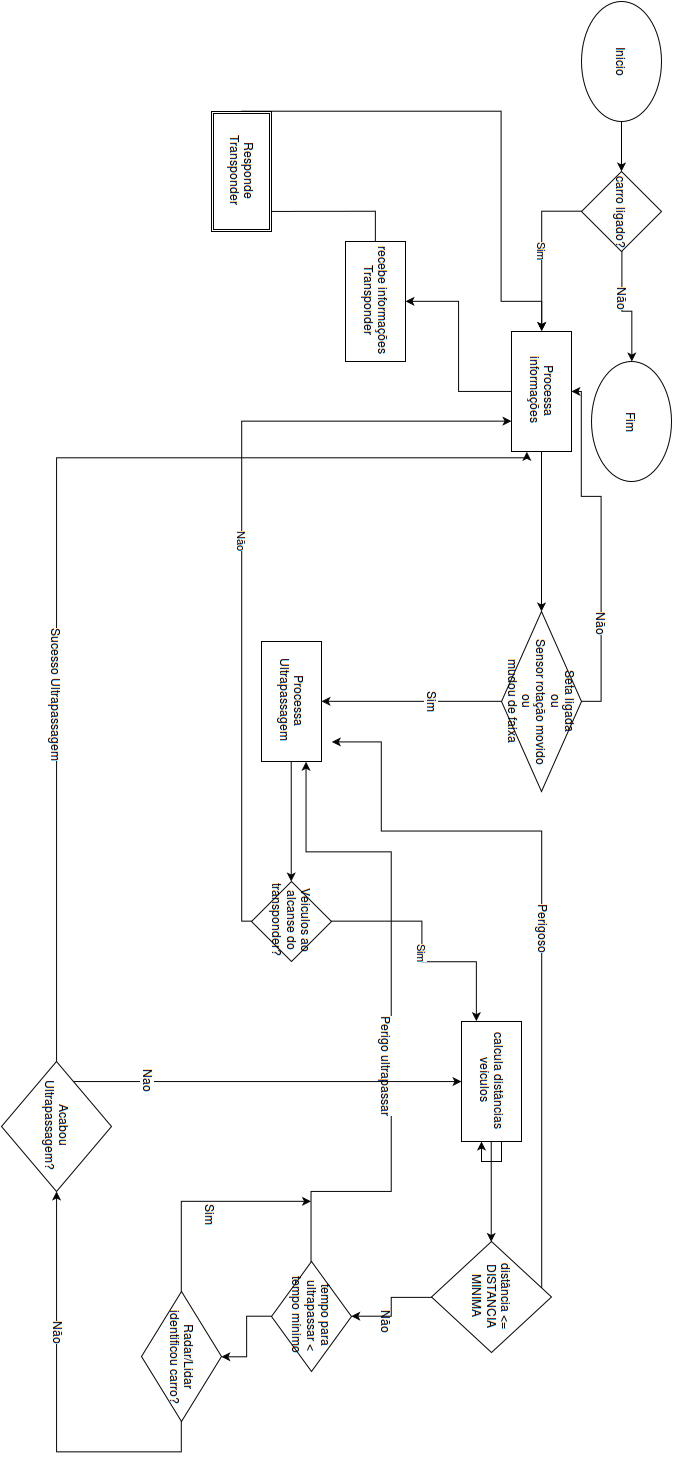
\includegraphics[width=200px, scale=1, angle=90]{figuras/func_soft}
  \caption{Fluxograma de funcionamento geral do Software}
\label{fig:func_soft}
\end{figure}

\section {Interface}

Dado o contexto do problema o qual o CIAC propõe resolver, para a construção de um dispositivo que se adeque bem a atender os requisitos de alertar o motorista, é necessário um estudo de campo e avaliações sobre o uso dos outros componentes eletrônicos no carro. Visto que a poluição visual ao motorista reduz a atenção do condutor à pista. Tendo este ponto inicial para trabalho, é de grande interesse buscar métodos de avaliação do conteúdo disposto na tela do dispositivo.

\subsection{A metodologia}

A construção dos protótipos para esta solução exige que a equipe tenha que identificar e refinar requisitos a cada interação, além de construir versões mais elaboradas a cada vez que se é feita uma nova avaliação do usuário sobre o protótipo mais atual. Tendo em vista tais necessidades o ciclo de vida adotado será o ciclo de vida Simples, cuja pesquisa está nos apêndices, embora pelo limite de tempo do projeto, a etapa de construção de uma versão interativa dos protótipos avaliados pelo usuário final não foi realizada.

Dessa forma, as etapas para a construção da solução de interação humano computador foram: Identificar necessidades e definir quais serão atendidas pelo projeto, design dos protótipos de baixa e alta fidelidade e avaliação do público-alvo.
    
\subsection{Heurística utilizada}

Na construção dos protótipos foram utilizadas as seguintes Heurísticas, pois elas adequam-se ao contexto do dispositivo a ser construído dentre as 10 apresentadas nos apêndices, conferindo ao usuário somente as informações necessárias para a funcionalidade.

Dentre as 10 Heurísticas apresentadas, foram selecionadas 5 que são elementares para que a interface de não atraia a atenção do motorista constantemente removendo a atenção do trânsito. São elas:

\begin{enumerate}
	\item Visibilidade de Status do Sistema
	\item Relacionamento entre a interface do sistema e o mundo real
	\item Consistência e padrões
	\item Estética e design minimalista
	\item Ajuda e documentação
\end{enumerate}

Estas Heurísticas foram utilizadas para a construção do protótipo de baixíssima fidelidade, apenas para a construção dos protótipos de baixa e alta fidelidade. Visto que o protótipo de baixíssima fidelidade foi elaborado apenas para criar o conceito inicial da tela da aplicação.

\subsection{Abordagem para construção de protótipos}

 Dadas as duas possíveis abordagens para a avaliação dos protótipos, o método de avaliação heurística e o analítico, foi determinado que o melhor método de avaliação a ser utilizado é o analítico, visto que é o mais prático de se implementar, levando-se em consideração o contexto do projeto, além de que a avaliação heurística para ser atestada deve ser avaliada por especialistas em interação humano computador, enquanto a primeira esta validação é realizada diretamente com os futuros usuários.

Para realização das perguntas para avaliação do protótipo desenvolvido, utilizou-se o modelo da carta de consentimento presente nos apêndices no qual, serve para atestar que o participante está ciente do tipo de pesquisa a ser realizada e permite a utilização de suas respostas como índices para avaliação do protótipo do produto.

Assim, com base nas respostas dos usuários, que podem ser consultadas nos apêndices, foi elaborado o protótipo final de alta fidelidade para a interface de comunicação direta com o usuário.

\begin{figure}[h!]
  \centering
  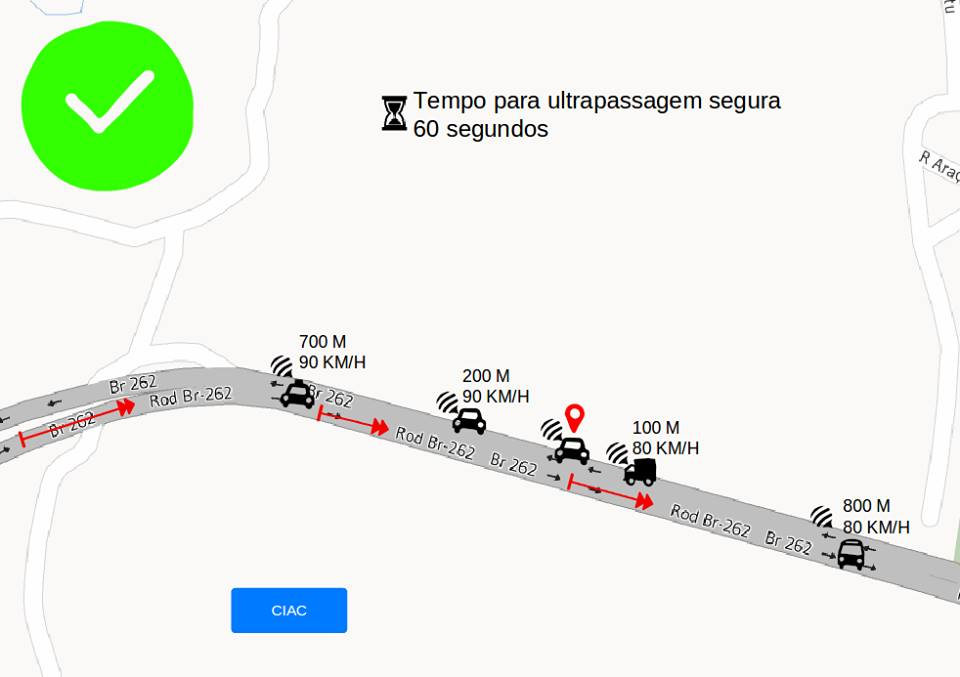
\includegraphics[width=400px, scale=1]{figuras/alta1}
  \caption{Protótipo de alta fidelidade 1}
\label{fig:alta1}
\end{figure}	

\begin{figure}[h!]
  \centering
  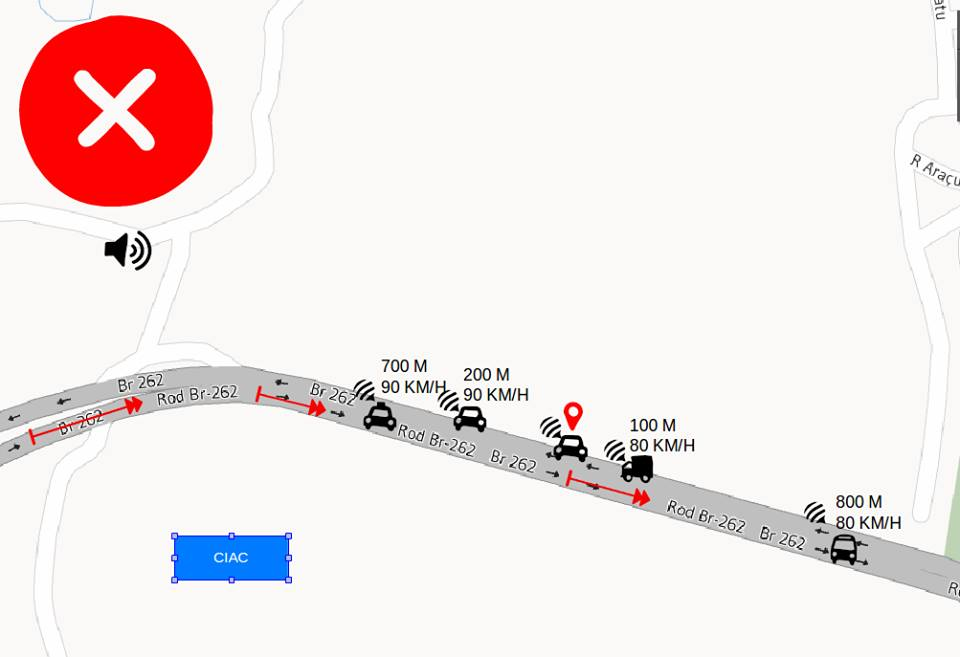
\includegraphics[width=400px, scale=1]{figuras/alta2}
  \caption{Protótipo de alta fidelidade 2}
\label{fig:alta2}
\end{figure}	

\subsection{Futuras melhorias propostas}

Para futuras construções de protótipos a serem projetados há a possibilidade de aumentar o escopo do projeto e adicionar as melhorias no produto:

\begin{itemize}
	\item Adicionar uma tela mais interativas onde o usuário possa interagir com ela e remover ou adicionar os veículos.
	\item Um menu com opções onde possa selecionar as opções que ele deseja visualizar.
	\item Botão com a possibilidade de visualizar as imagens geradas pela câmera utilizada pelo sistema.
	\item Gravar as imagens geradas em um armazenador de dados externo.
	\item Integrar o atual sistema com a função de GPS por meio de um botão.
\end{itemize}